\chapter{Introduction}
\label{sec:introduction}


A fundamental test of lepton universality in the electroweak sector is to measure the branching fractions of the W boson.  The most precise measurements of these quantities were measured at LEP~\cite{Schael:2013ita} and the results of all four experiments are combined to form the world averages~\cite{Patrignani:2016xqp}.  The values measured at each experiment and their combined values are shown in figure~\ref{fig:introduction:wbr}.

\begin{figure}[ht]
    \centering
    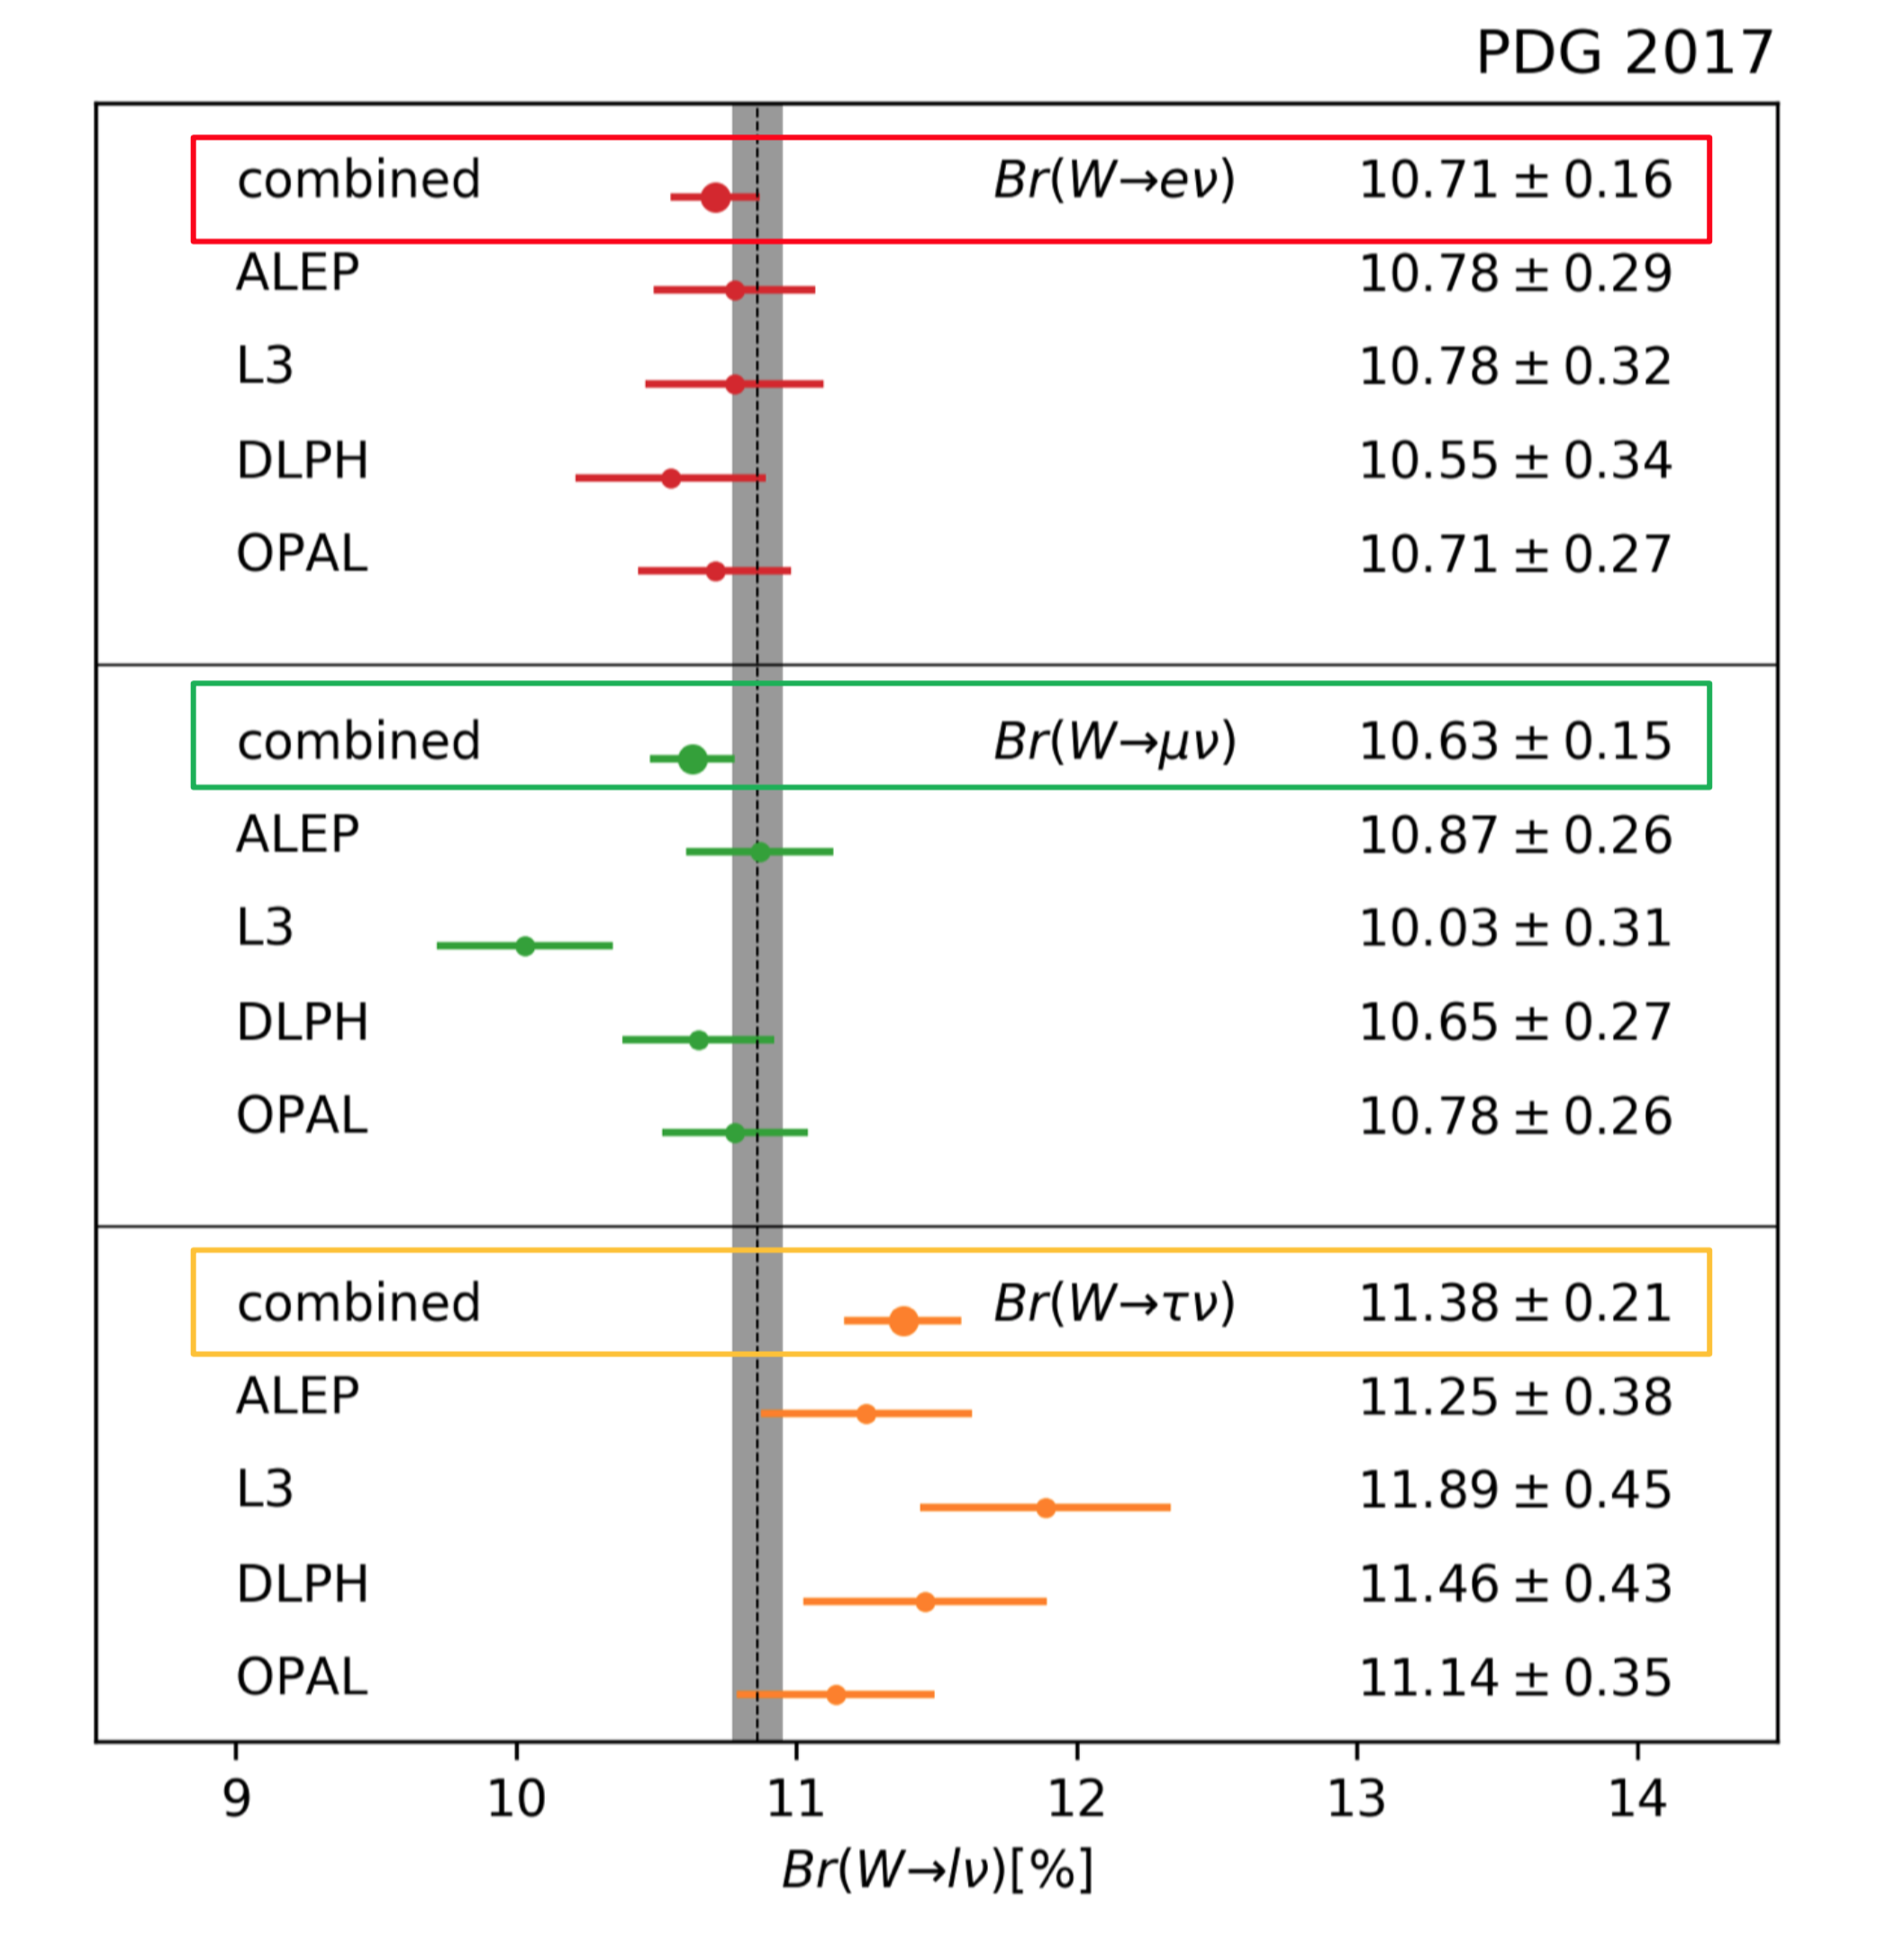
\includegraphics[width=0.6\textwidth]{chapters/Introduction/figures/wdecay.png}
    \caption{Measured leptonic and inclusive hadronic W branching fractions from LEP.}
    \label{fig:introduction:wbr}
\end{figure}


These measurements show a $\sim 2.6~\sigma$ difference between the tau branching fraction in the case that the fit is carried out assuming lepton universality and the case that each of the branching fractions can vary independently.  This motivates measuring the branching fractions more precisely.  Because of the large number of \ttbar events produced at the LHC, it is possible to select a high statistics, high purity dataset containing two W boson decays which can be used to precisely measure the W branching fractions.  


In this analysis, $35.9\fbinv$ of data collected by CMS at $\sqrt{s} =13$ TeV during the 2016 run of the LHC are analyzed by selecting events consistent with the decay of pair-produced top quarks or W bosons are selected.  Final states resulting from either one or both of the W bosons decaying leptonically are considered.  To collect these events, single lepton triggers are used thus requiring that the final state must contain at least one prompt electron or muon. 

Estimation of the values of the W branching fractions is carried out based on two approaches: 

\begin{itemize}
    \item maximum likelihood estimation (MLE), binning the data based on the number of b-tags and channel-dependent kinematic information. This will be referred to as the \emph{shape analysis}.
    \item a semi-analytic approach that constructs ratios of yields in the various channels in a manner that mimics a direct construction of the branching fraction.  This approach does not use kinematic shape information, but does divide channels based on the number of b tags. This will be referred to as the \emph{counting analysis}.
\end{itemize}